\documentclass[12pt]{article}
\usepackage[top=1in,bottom=1in,left=1in,right=1in]{geometry}
\usepackage{alltt}
\usepackage{array}	
\usepackage{graphicx}
\usepackage{tabularx}
\usepackage{verbatim}
\usepackage{setspace}
\usepackage{listings}
\usepackage{amssymb,amsmath, amsthm}
\usepackage[
    pdfborder={0 0 0},
]{hyperref}

\title{Concordia University\\
Department of Computer Science and Software Engineering\\
\textbf{SOEN 331 - S and U\\Introduction to Formal Methods\\for Software Engineering}\\
\ \\
\textbf{Assignment 3 - Solutions}\\
Extended Finite State Machines\\
\textbf{Team 19 - Section U}}
\author{
	\textbf{Samuel Boaknin}\\
	\texttt{40009692}
	\and
	\textbf{Ryan Leyland}\\
	\texttt{40015165}
	\and
	\textbf{Saleha Tariq}\\
	\texttt{40006997}
	\and
	\textbf{Meng Susana Ung}\\
	\texttt{40099729}
}
\date{Due Date: April 9, 2021}
\begin{document}
\begin{spacing}{1.5}

\maketitle

\section{Washing Machine formal specification}

\noindent The EFSM of the washing machine is the tuple $S = (Q, \Sigma_1, \Sigma_2, q_0, \Lambda)$, where\\
\noindent $Q = \{\text {off, on}\}$\\
\noindent $\Sigma_1 = \{\text {turn on, turn off}\}$\\
\noindent $\Sigma_2 = \{\text {beep, turn light off}\}$\\
\noindent $q_0: \text{off}$\\
%\noindent $V: \{\}$\\
\noindent $\Lambda$: Transition specifications\\
\indent 1. $\rightarrow off $\\
\indent 2. $off \xrightarrow {\text { turn on }} on$\\
\indent 3. $on \xrightarrow {\text { turn off / (beep; turn light off) }} off$\\

\noindent As $on$ is a composite state, it is defined as the tuple $S = (Q, \Sigma_1, \Sigma_2, q_0, \Lambda)$, where\\
\noindent $Q = \{\text {operating, servicing}\}$\\
\noindent $\Sigma_1 = \{\text {after (10 s), service signal [idle], machine fixed}\}$\\
\noindent $\Sigma_2 = \{\text {blinking, long beep}\}$\\
\noindent $q_0: \text{operating}$\\
%\noindent $V: \{\}$\\
\noindent $\Lambda$: Transition specifications\\
\indent 1. $\xrightarrow {\text { after (10 s) / (blinking; long beep) }} operating$\\
\indent 2. $operating \xrightarrow {\text { service signal [idle] }} service$\\
\indent 3. $service \xrightarrow {\text { machine fixed }} operating$\\
\newpage

\noindent As $operating$ is a composite state, it is defined as the tuple $S = (Q, \Sigma_1, \Sigma_2, q_0, \Lambda)$, where\\
\noindent $Q = \{\text {idle, standby, active}\}$\\
\noindent $\Sigma_1 = \{\text {light on, start signal or finish button, power off, power on, completion, cancel, cancel [setting]}\}$\\ 
\noindent $\Sigma_2 = \{\text {turn light on, clear settings, unlock door}\}$\\
\noindent $q_0: \text{idle}$\\
%\noindent $V: \{\}$\\
\noindent $\Lambda$: Transition specifications\\
\indent 1. $\xrightarrow {\text { light on / turn light on }} idle$\\
\indent 2. $idle \xrightarrow {\text { start signal or finish button }} active$\\
\indent 3. $active \xrightarrow {\text { cancel }} idle$\\
\indent 4. $active \xrightarrow {\text { completion / unlock door }} idle$\\
\indent 5. $active \xrightarrow {\text { cancel [setting] / clear settings }} idle$\\
\indent 6. $active \xrightarrow {\text { power off }} standby$\\
\indent 7. $standby \xrightarrow {\text { power on }} active$\\\\
\noindent The UML state diagram is shown in Figure~\ref{fig:wm-fig1}.\\
\newpage

\noindent As $active$ is a composite state, it is defined as the tuple $S = (Q, \Sigma_1, \Sigma_2, q_0, V, \Lambda)$, where\\\\
\noindent $Q = \{\text {setting, washing, rinse, spin}\}$\\
\noindent $\Sigma_1 = \{\text {start-finish, after (3 min), after (2 min)}\}$\\ 
\noindent $\Sigma_2 = \{\text {lock door}\}$\\
\noindent $q_0: \text{setting}$\\
\noindent $V: \text{ door = \{open, closed\} }$\\
\noindent $\Lambda$: Transition specifications\\
\indent 1. $\xrightarrow {} setting$\\
\indent 2. $setting \xrightarrow {\text { [door is closed] start-finish / lock door }} washing $\\
\indent 3. $washing \xrightarrow {} rinse$\\
\indent 4. $rinse \xrightarrow {\text { after (3 min) }} spin$\\
\indent 5. $spin  \xrightarrow {\text { after (2 min)}}$\\

\noindent The EFSM of the $washing$ state is the tuple $S = (Q, \Sigma_1 q_0, V, \Lambda)$, where\\\
\noindent $Q = \{\text {heating, longwash, shortwash}\}$\\
\noindent $\Sigma_1 = \{\text {after (2 min), after (30 min), after (10 min)}\}$\\ 
\noindent $q_0: \text{heating}$\\
\noindent $V: \text{ currentTemp, desiredTemperature: } \mathbb{R}, \text{ mode = \{short, long\}}$\\
\noindent $\Lambda$: Transition specifications\\
\indent 1. $\xrightarrow {} heating$\\
\indent 2. $heating \xrightarrow {\text { [ ct $<$ desiredTemp] after (2 min)}} heating $\\
\indent 3. $heating \xrightarrow {\text { [ ct $\geq$ desiredTemp] [mode is long] after (2 min)}}  longwash$\\
\indent 4. $heating \xrightarrow {\text { [ ct $\geq$ desiredTemp] [mode is short] after (2 min)}}  shortwash$\\
\indent 5. $longwash  \xrightarrow {\text { after (30 min)}}$\\
\indent 5. $shortwash  \xrightarrow {\text { after (10 min)}}$\\

\noindent The UML state diagram is shown in Figure~\ref{fig:wm-fig2}.\\\\
\newpage

\section{UML state diagrams}

\begin{figure}[h!]
	\centering
		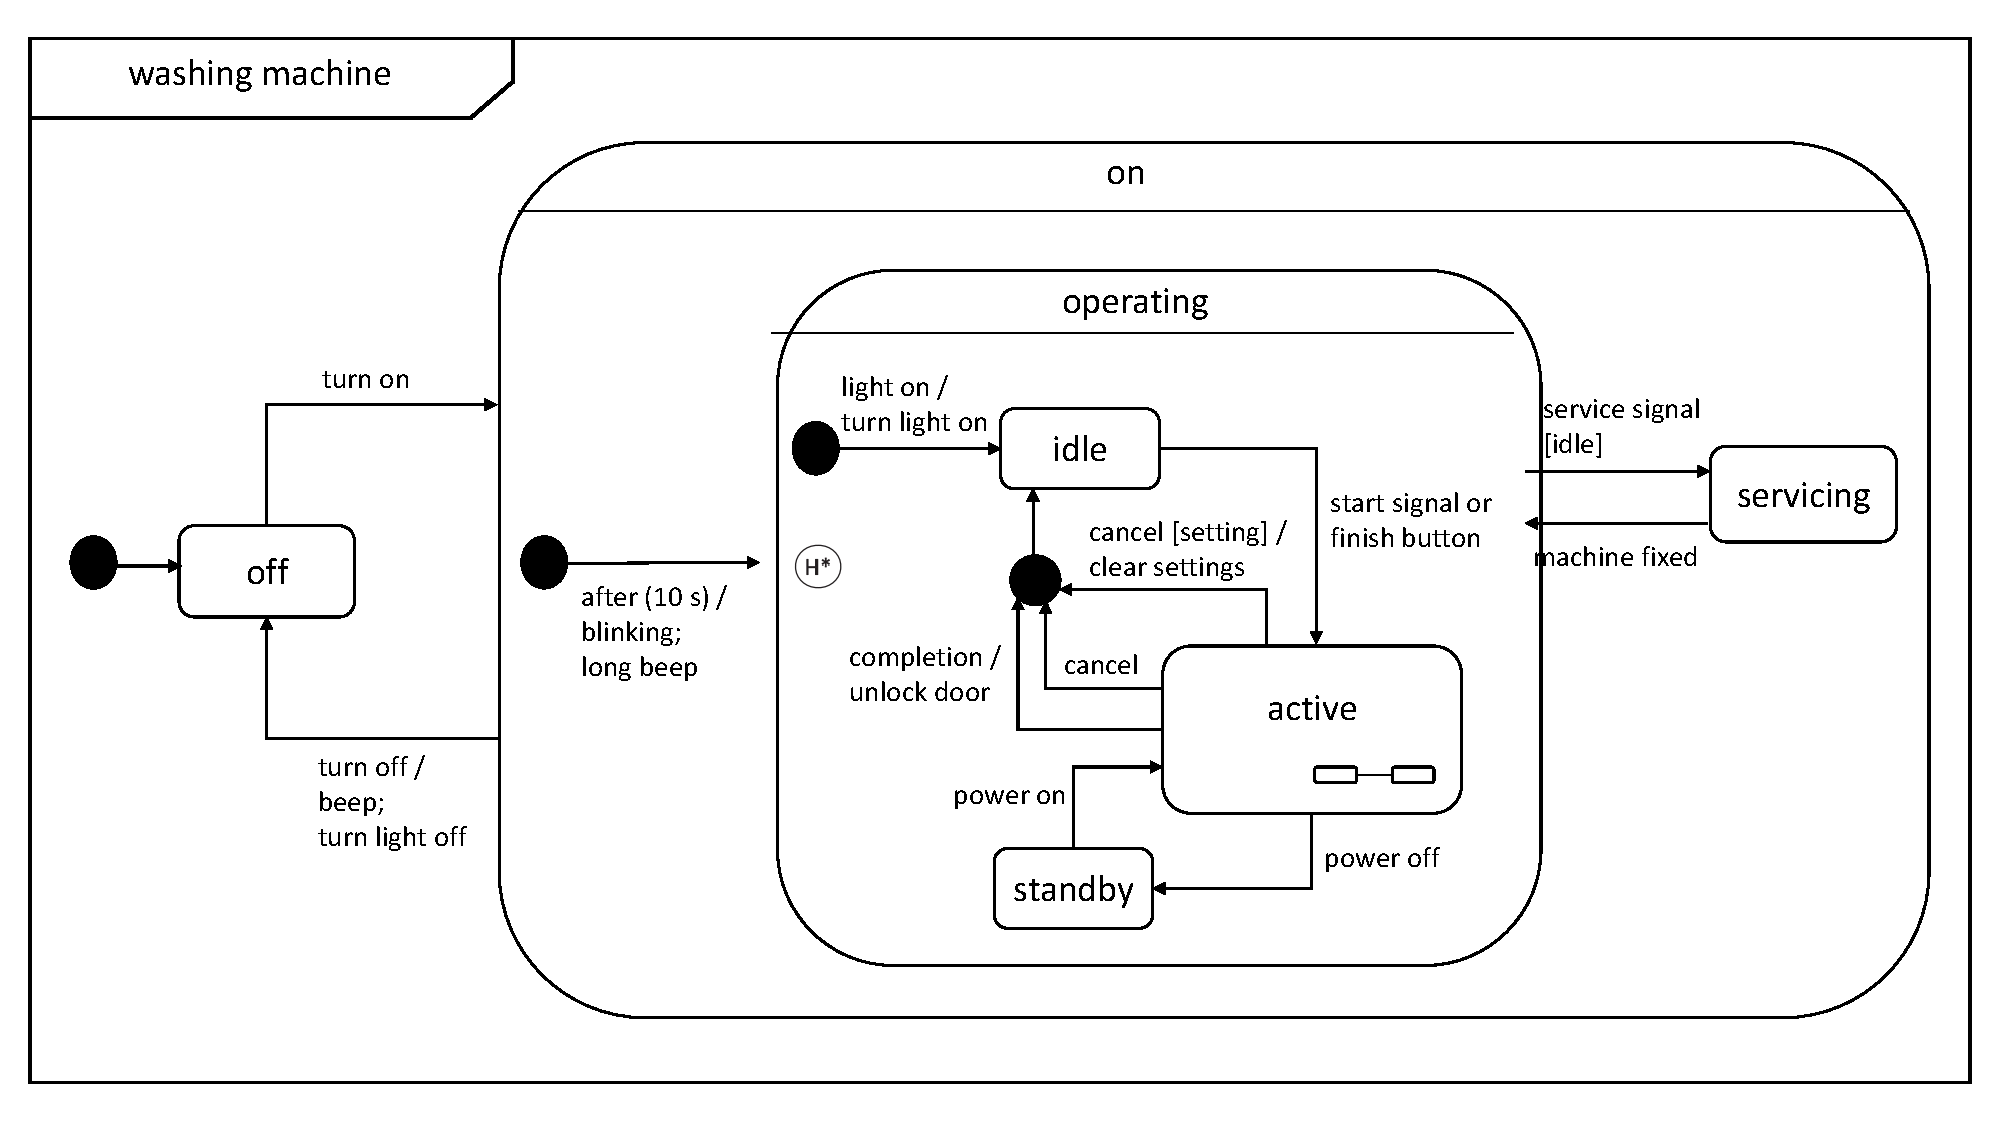
\includegraphics[page=1,width=1\textwidth]{./figures/updatedSecondDraft.pdf}
		  \caption{Washing Machine}
  \label{fig:wm-fig1}
\end{figure}

\begin{figure}[h!]
	\centering
		\includegraphics[page=2,width=0.95\textwidth]{./figures/updatedSecondDraft.pdf}
		  \caption{Washing Machine (Active state) }
  \label{fig:wm-fig2}
\end{figure}

\end{spacing}
\end{document}
